\documentclass[10pt]{article}
\usepackage{amsmath}
\usepackage{graphicx}
\usepackage{mathrsfs}
\usepackage[margin=0.0in]{geometry}
\begin{document}
	Equations:
	
	Generalised SWWE equations (when $\epsilon = 0$ we get SWWE, for other values we have equations that smooth out discontinuities). Generalised SWWE is more in line with what they represent, since they have same wavespeeds of SWWE and recreate them except without discontinuitites.
	
	They are:
We solve the following form of the regularised Serre equation
\begin{subequations}
	\begin{gather}
	\dfrac{\partial h}{\partial t} + \dfrac{\partial (uh)}{\partial x} = 0
	\label{eq:gSV_Ga}
	\end{gather}
	\begin{gather}
	\dfrac{\partial G}{\partial t} + \dfrac{\partial }{\partial x} \left[ uG + \dfrac{gh^2}{2} - \epsilon h^2\left ( 2 h \dfrac{\partial u}{\partial x} \dfrac{\partial u}{\partial x} + gh \dfrac{\partial^2h}{\partial x^2} +\dfrac{g}{2} \dfrac{\partial h}{\partial x}\dfrac{\partial h}{\partial x} \right ) \right]= 0
	\label{eq:gSV_Gb}
	\end{gather}
	\label{eq:gSV_G}
\end{subequations}
where
\begin{gather*}
G = uh - \epsilon \dfrac{\partial }{\partial x} \left (h^3 \dfrac{\partial u}{\partial x} \right )
\end{gather*}

I have allowed $\epsilon$ to vary in space and time to give $\epsilon(x,t)$. I then forced a solution by introducing $h^*$,$u^*$,$G^*$, $\epsilon^*$ and solving the forced version of these equations:
	
	\[
	\frac{\partial h}{\partial t} + \frac{\partial (uh)}{\partial x} = \frac{\partial h^*}{\partial t} + \frac{\partial (u^*h^*)}{\partial x}
	\]
	\begin{multline}	
	\frac{\partial G}{\partial t} + \frac{\partial }{\partial x} \left ( Gu + \frac{gh^2}{2}  - \epsilon^* h^2\left ( 2 h \dfrac{\partial u}{\partial x} \dfrac{\partial u}{\partial x} + gh \dfrac{\partial^2h}{\partial x^2} +\dfrac{g}{2} \dfrac{\partial h}{\partial x}\dfrac{\partial h}{\partial x} \right ) \right )\\ = \frac{\partial G^*}{\partial t} + \frac{\partial }{\partial x} \left ( G^*u^* + \frac{g(h^*)^2}{2} - \epsilon^* (h^*)^2\left ( 2 h^* \dfrac{\partial u^*}{\partial x} \dfrac{\partial u^*}{\partial x} + gh^* \dfrac{\partial^2h^*}{\partial x^2} +\dfrac{g}{2} \dfrac{\partial h^*}{\partial x}\dfrac{\partial h^*}{\partial x} \right ) \right )
	\end{multline}
	
	where RHS is calculated analytically and LHS is approximated numerically using $\text{FDVM}_2$ (second-order finite difference volume method)
	
	I used 
	\[h^* = a_0 + a_1 \exp \left[ \dfrac{\left(x - a_2 t\right)^2}{2a_3}\right]\]
	\[u^* = a_4 \exp \left[ \dfrac{\left(x - a_2 t\right)^2}{2a_3}\right]\]
	\[\epsilon^* = a_5 \cos\left(a_7(x - a_6 t)\right) \]
	
	\[
	G^* = u^*h^* - \epsilon^* \frac{\partial }{\partial x} \left ( \dfrac{(h^*)^3}{3} \frac{\partial u^*}{\partial x} \right ).
	\]
	
	When solving for $u$ using $h,G$ I supplied the analytic value of $\epsilon^*$
	
	
	With
	$x \in \left[-50,100\right]$\\
	Number of cells varied like so $n = 100\times2^k$ with $k \in \left[0,9\right]$\\
	$$\Delta x = \frac{100 - (-50)}{n}$$
	$$\frac{\Delta t}{\Delta x} = \frac{Cr}{a_2 + a_4 + \sqrt{g(a_0 + a_1)}}$$
	$Cr = 0.5$, 
	$g =   9.81 $,  
	$a0 =   1.0$,   
	$a1 =   0.5$,   
	$a2 =   5.0$,    
	$a3 =   20.0$,    
	$a4 =   0.3$,
	$a5 =   2.0$,
	$a6 =   -0.5$,
	$a7 =   \frac{\pi}{125}$
	
	Results:
	 
	I have plotted results for various $\epsilon$ values together to demonstrate method can handle both extremes (SWWE and Serre) as well as inbetween values.
	
	Example Solutions

	\begin{figure}[h!]
		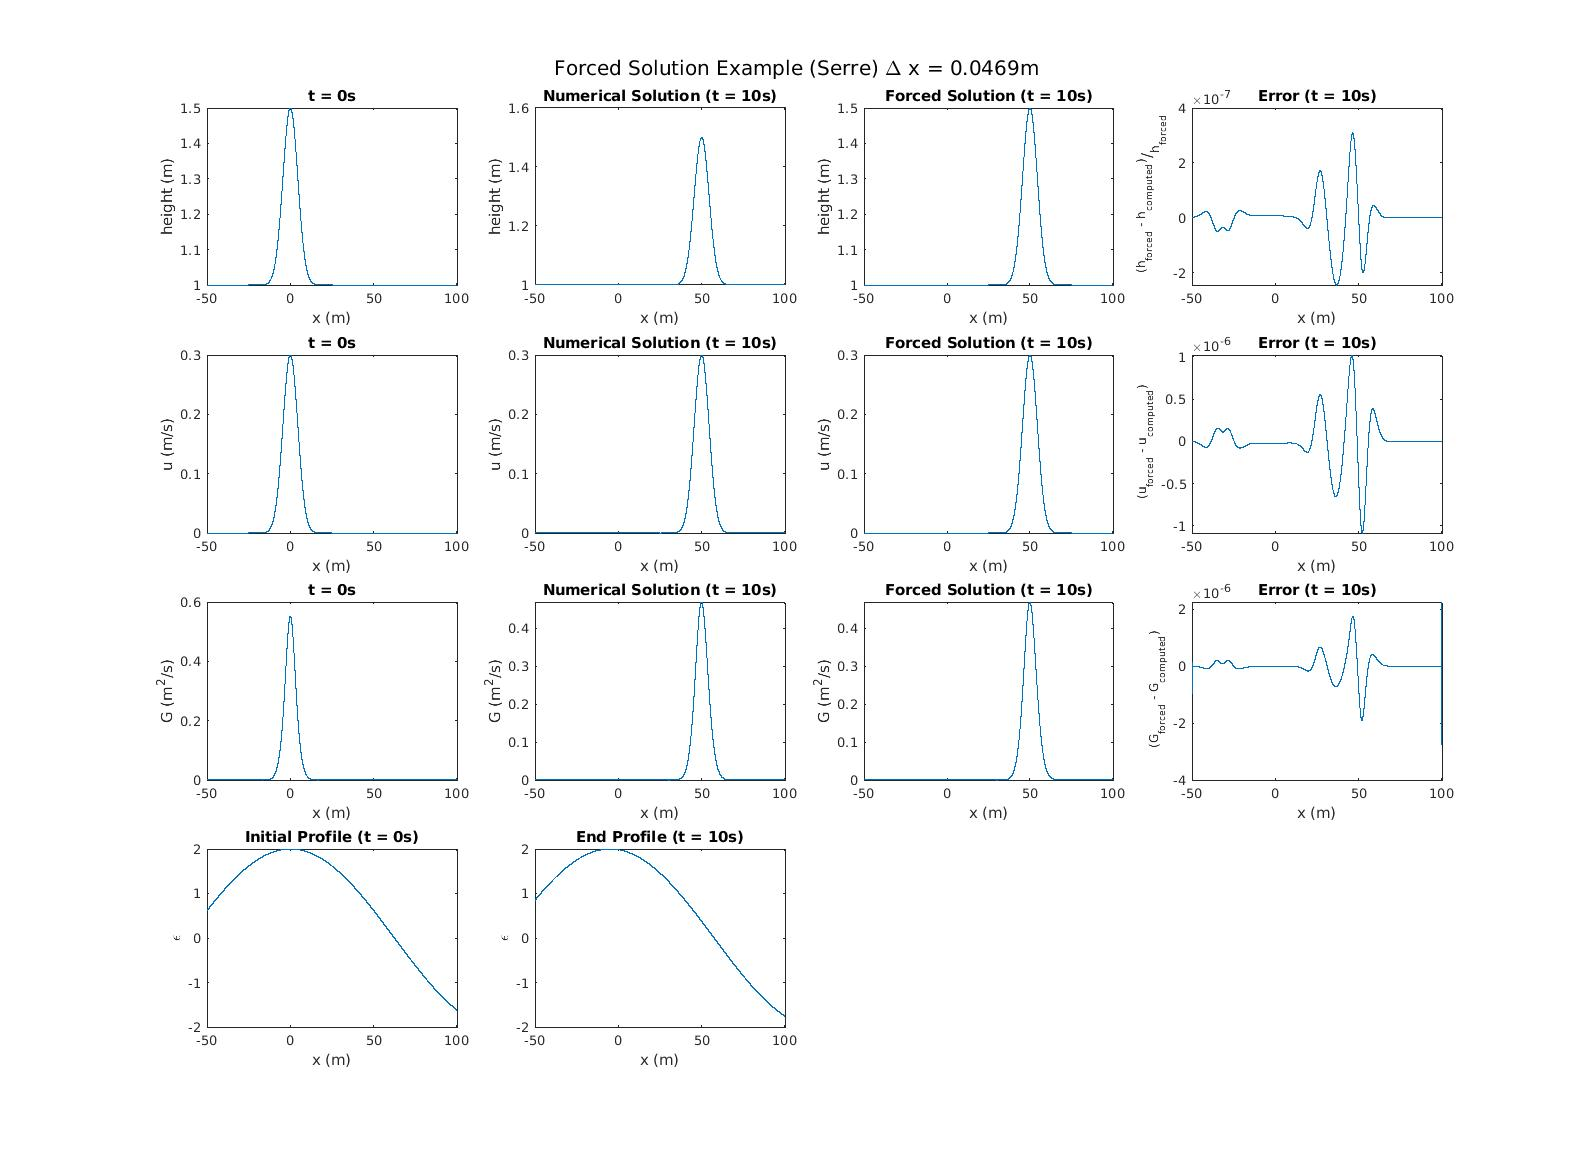
\includegraphics[width=23.0cm]{ExampleResults.jpg}
		\caption{Example results }
	\end{figure}

	
	Convergence with second order slope shown
	
	\begin{figure}[h!]
		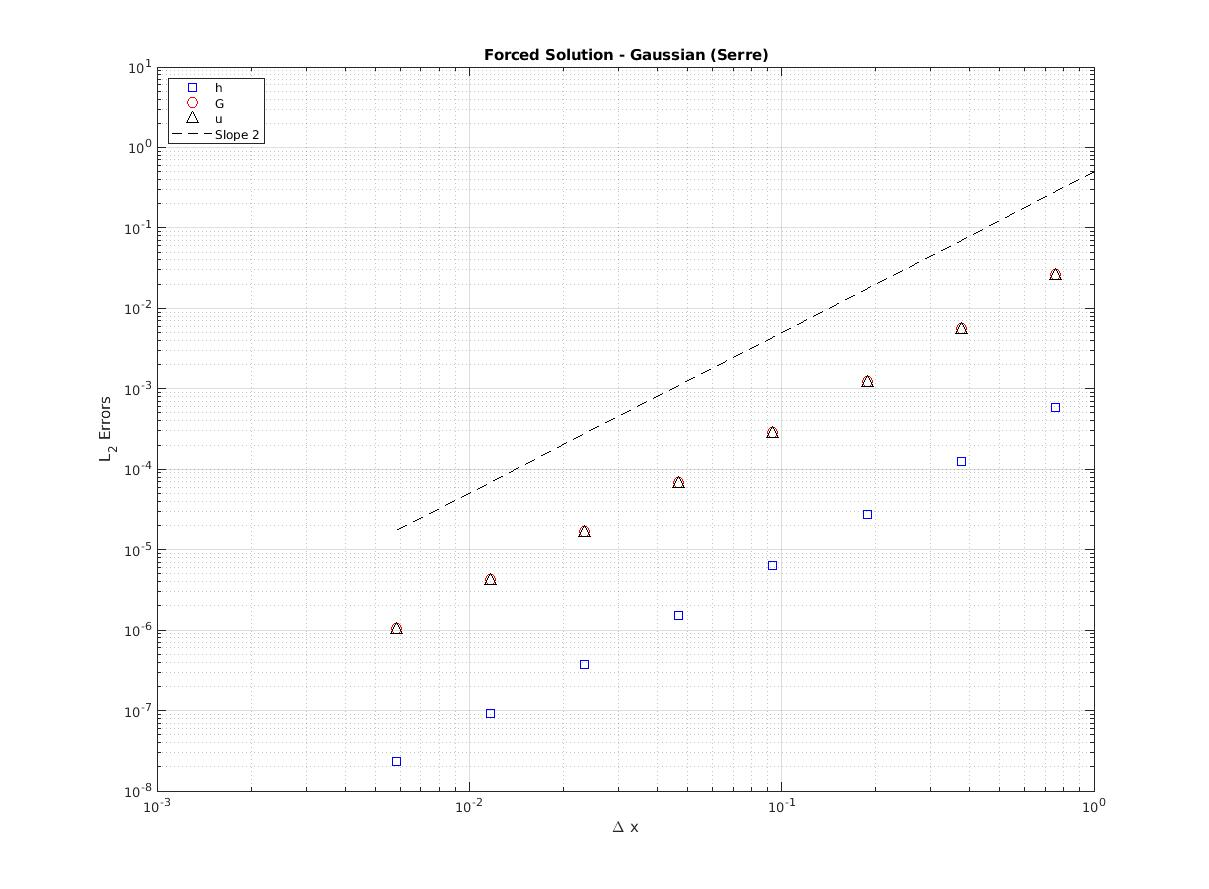
\includegraphics[width=23.0cm]{NormResults.jpg}
		\caption{$L_2$ norms }
	\end{figure}

	Discussion:
	         hir = hbc(i) + cdhi/2
	Gir = Gbc(i) + cdGi/2
	uir = (ubc(i+1)+ubc(i))/2
	duir = (ubc(i+1) - ubc(i)) /dx
	dhir = (hbc(i+1) - hbc(i)) /dx
	ddhir = (hbc(i+2)  - hbc(i+1) - hbc(i) + hbc(i-1) )/(2*dx**2)
	
	I was only able to get this to work, by not limiting and using the reconstructions:
	
	for $h$ and $G$ I used
	\[q^-_{j+1/2} = q_j + \frac{q_{j+1} - q_{j-1}}{4} \]
	\[q^+_{j+1/2} = q_{j+1} - \frac{q_{j+2} - q_{j}}{4} \]
	
	for $h_x$ and $u_x$ I used
	\[\left(\frac{\partial q}{\partial x}\right)^\pm_{j+1/2} = \frac{q_{j+1} - q_j}{\Delta x}\]
	
	for $h_{xx}$ I used
\[\left(\frac{\partial^2 h}{\partial x^2}\right)^\pm_{j+1/2} = \frac{q_{j+2} - q_{j+1} - q_{j} +   q_{j-1}}{2 \Delta x^2}\]	

	It still satisfactorily shows that we can solve the equations with $\epsilon$ varying. Annyoing I couldn't get it to work with the method I want to use which would be the minmod limiting on $h$ and $G$ with the following approximations to the derivatives (which are second-order forward and backward approximations):
	
	for $h_x$ and $u_x$:
	\[\left(\frac{\partial q}{\partial x}\right)^-_{j+1/2} = \frac{2q_{j} - 3q_{j-1} + q_{j-2}}{\Delta x} \]
	\[\left(\frac{\partial q}{\partial x}\right)^+_{j+1/2} = \frac{-2q_{j+1} + 3q_{j+2} - q_{j+3}}{\Delta x} \]
	
	for $h_{xx}$
	\[\left(\frac{\partial^2 h}{\partial x^2}\right)^-_{j+1/2} = \frac{5q_j -13 q_{j-1} + 11 q_{j-2} - 3 q_{j-3}}{2 \Delta x^2}\]
	\[\left(\frac{\partial^2 h}{\partial x^2}\right)^+_{j+1/2} = \frac{5q_{j+1} -13 q_{j+2} + 11 q_{j+3} - 3 q_{j+4}}{2 \Delta x^2}\]		
	
  
\end{document}